
% Copyright (c) 2015 - 2020 Mario Mlačak, mmlacak@gmail.com
% Licensed and published as Public Domain work.

% Miranda's veil chapter ==============================================
\chapter*{Miranda's veil}
\addcontentsline{toc}{chapter}{Miranda's veil}

\begin{flushright}
\parbox{0.8\textwidth}{
\emph{Under all that we think, lives all we believe, like the ultimate veil of our spirits. \\
\hspace*{\fill}{\textperiodcentered \textperiodcentered \textperiodcentered \hspace*{0.2em} Antonio Machado} } }
\end{flushright}

\noindent
Miranda's veil is chess variant which is played on 16 x 16 board, with
white and dark violet fields and light magenta and indigo pieces. In
algebraic notation, columns are enumerated from 'a' to 'p', and rows
are enumerated from '1' to '16'. A new piece is introduced, Wave.

\clearpage % ..........................................................
% Wave ****************************************************************

\section*{Wave}
\addcontentsline{toc}{section}{Wave}

\vspace*{-1.0ex}
\noindent
\begin{wrapfigure}[12]{l}{0.4\textwidth}
\centering
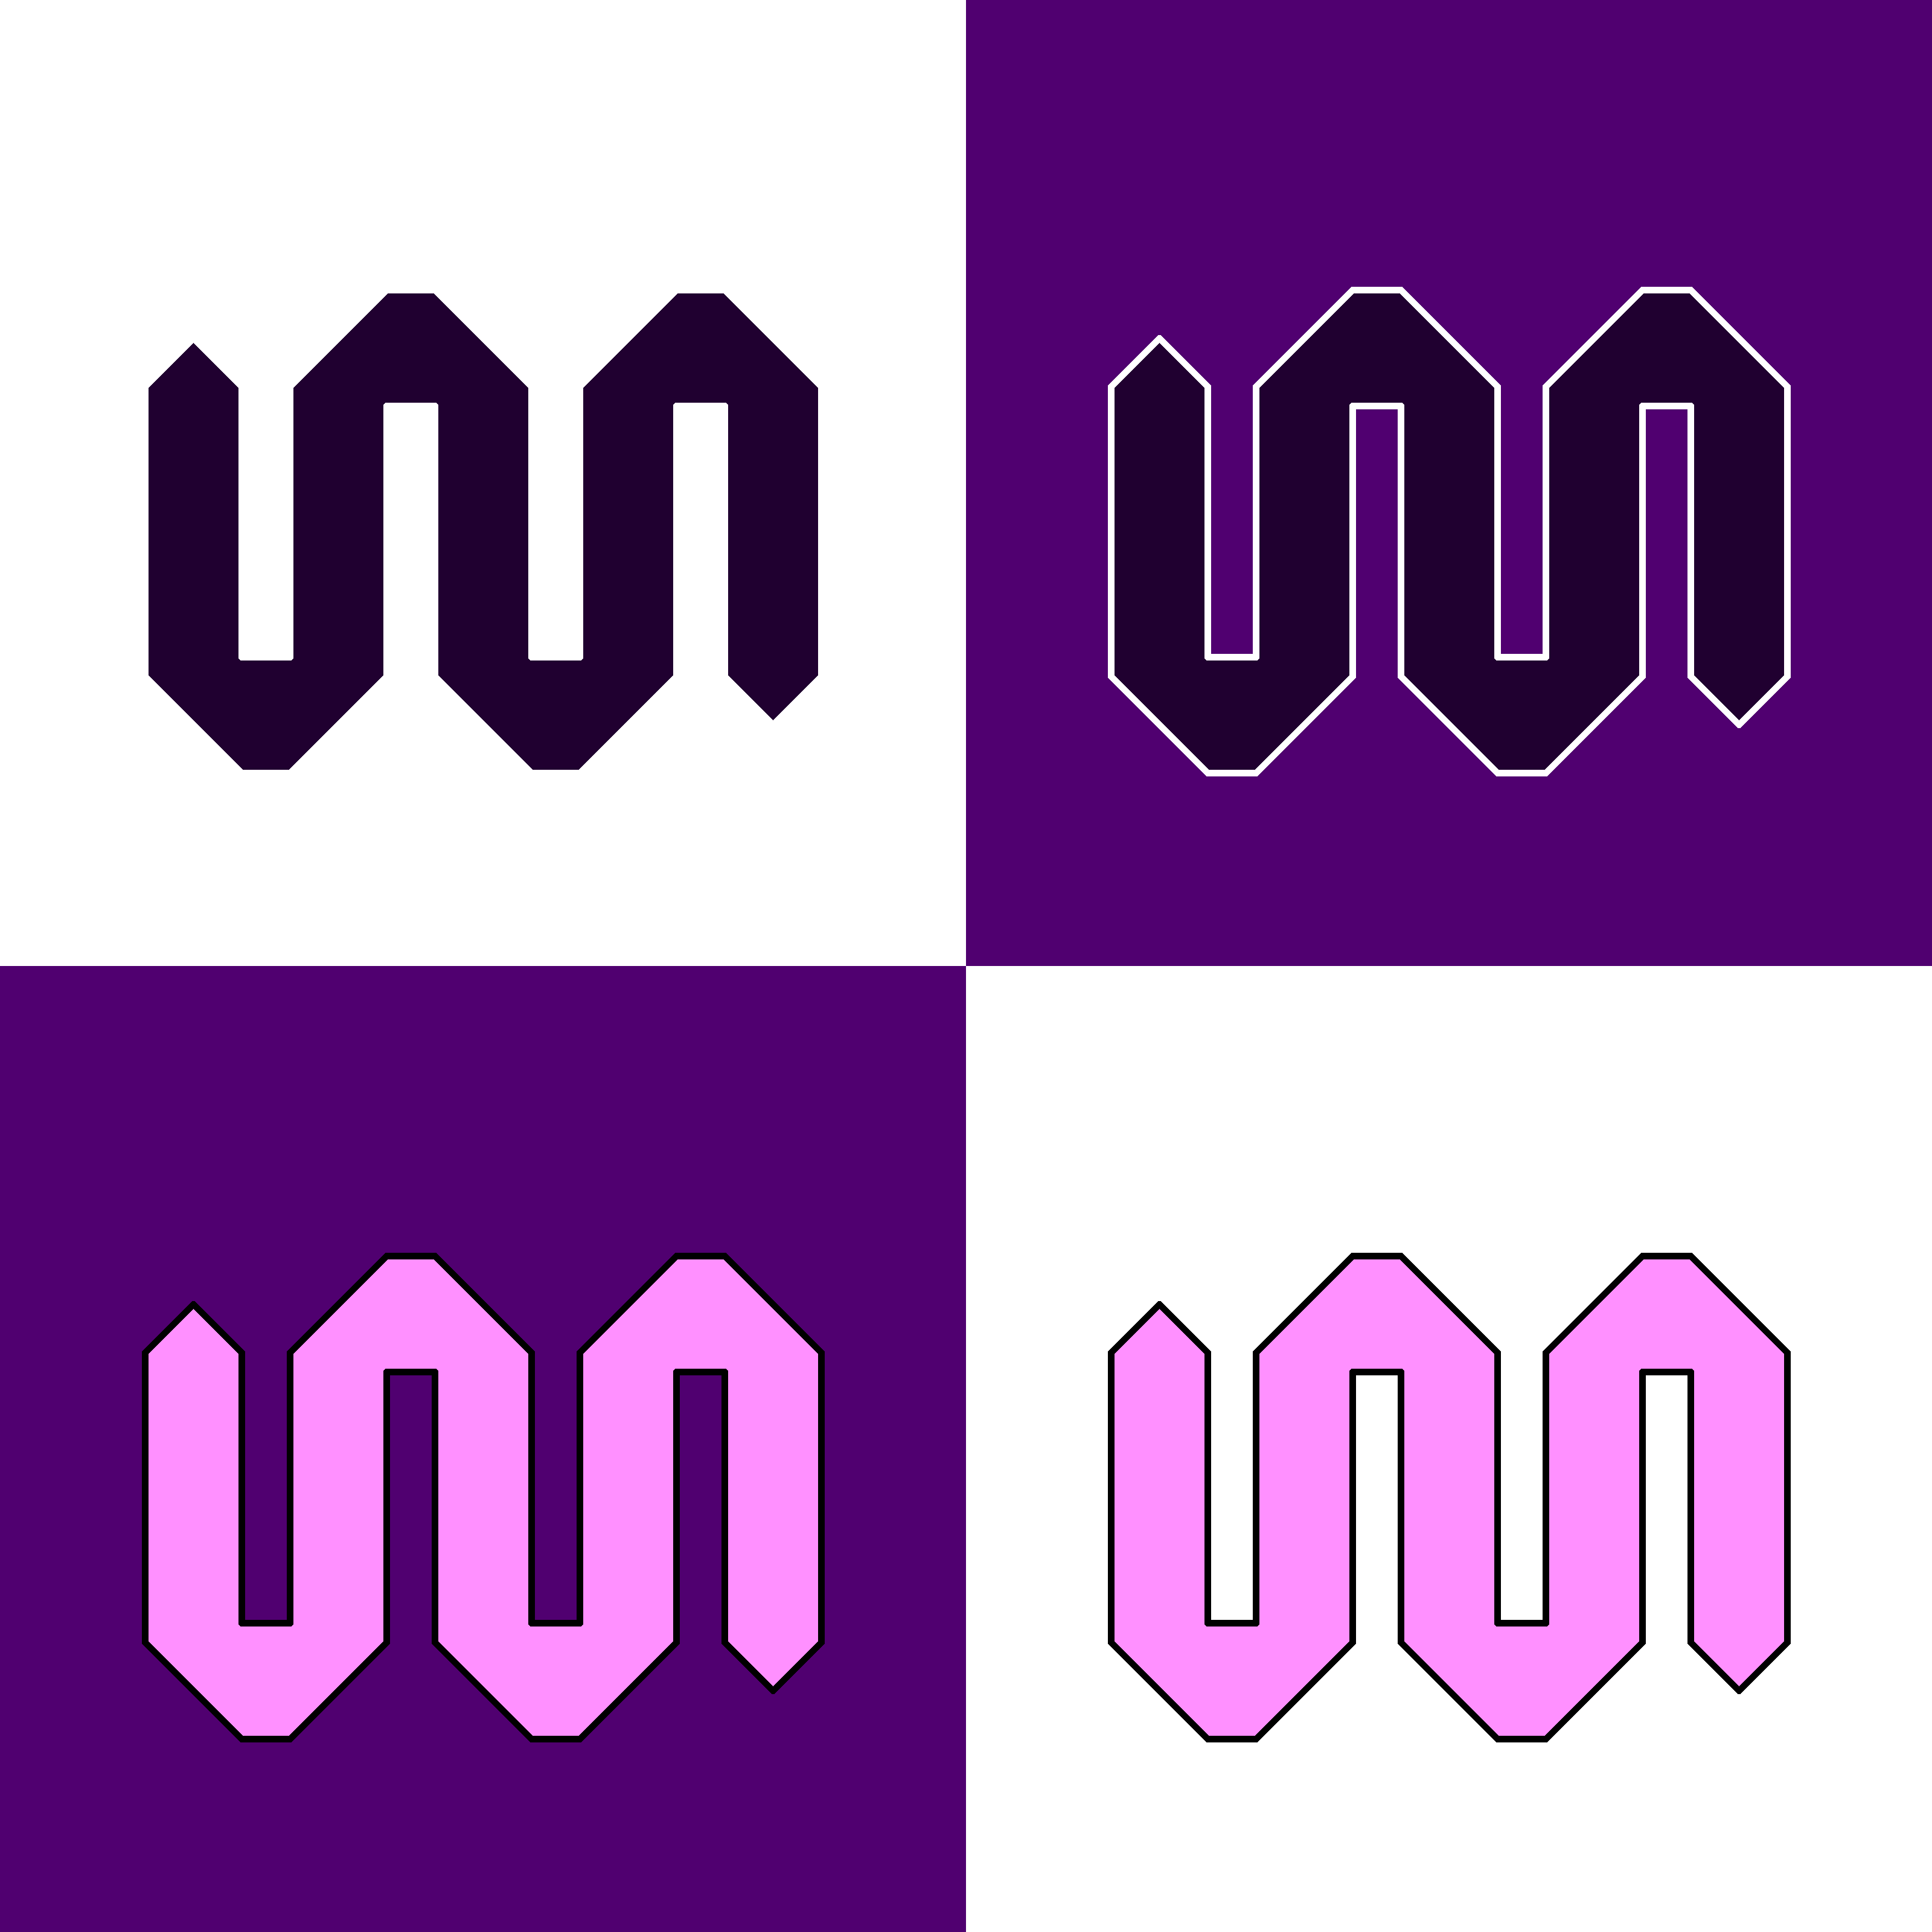
\includegraphics[width=0.4\textwidth, keepaspectratio=true]{pieces/10_wave.png}
\caption{Wave}
\label{fig:10_wave}
\end{wrapfigure}
Wave is passive piece, it has to be activated before it can move. Activation
is done in the same way as with Pyramid. Own piece has to capture field at
which Wave is located before Wave can move.

Wave can be activated even if activating piece has no momentum. Wave does not use
received momentum for moving, and isn't limited by it. Wave can move even if it
has no momentum. Wave can move past (pass "through") any piece, as if it isn't there.

After activation Wave moves like activating piece, over piece's step- or capture-
fields, depending where it was activated. Wave can make multiple steps, in the
same way activating piece does, even if activating piece can make only one. Note,
Wave can choose direction only on first 1 (or 2) step(s), which cannot be changed
later. Wave can step outside of a chessboard, and only has to end its ply on a
board. For details see
\hyperref[sec:Appendix/Movement of Wave]{Movement of Wave}.

Wave cannot capture any piece. Thus, Wave cannot neither check nor checkmate
opponent's King.

Wave can activate any own piece, except King, if it has momentum. Wave can
also activate other Wave, own or opponent's, even if it has no momentum. In
all cases, Wave transfers all received momentum to activated piece.

In algebraic notation symbol for Wave is 'W'.

\clearpage % ..........................................................
% Activation ----------------------------------------------------------

\subsection*{Activation}
\addcontentsline{toc}{subsection}{Activation}

\vspace*{-1.4\baselineskip}
\noindent
\begin{figure}[!h]
\includegraphics[width=1.0\textwidth, keepaspectratio=true]{examples/10_mv/scn_mv_01_wave_activation_init.png}
\caption{Activating Wave}
\label{fig:scn_mv_01_wave_activation_init}
\end{figure}

Own piece can activate own Wave by simply capturing a field at which that Wave
stands. Activated Wave receives any momentum activating piece had.

Here, Pegasus is about to activate Wave, and transfer to it all of 5 momentum,
collected by travelling over 5 fields.

\clearpage % ..........................................................

\vspace*{-2.1\baselineskip}
\noindent
\begin{figure}[!h]
\includegraphics[width=1.0\textwidth, keepaspectratio=true]{examples/10_mv/scn_mv_02_wave_activated.png}
\caption{Wave activated}
\label{fig:scn_mv_02_wave_activated}
\end{figure}

Activated Wave inherits way of moving from the activating piece. Activated Wave
does not spend received momentum for moving, and so Wave can be activated even if
activating piece has no momentum.

Here, Wave activated by Pegasus (now "in the air") moves like one, i.e. along one
chosen semi-diagonal.

\clearpage % ..........................................................

\subsubsection*{Activating pieces}
\addcontentsline{toc}{subsubsection}{Activating pieces}

\vspace*{-1.4\baselineskip}
\noindent
\begin{figure}[!h]
\includegraphics[width=1.0\textwidth, keepaspectratio=true]{examples/10_mv/scn_mv_03_pawn_pass_through.png}
\caption{Passing opponent's Pawn}
\label{fig:scn_mv_03_pawn_pass_through}
\end{figure}

Wave in its movement is not obstructed by any piece on chessboard, it can
"pass-through" any piece, as if it's not there.

Here, Wave cannot activate opponent's Pawn on its step-field, but it's not
hindered by that Pawn, and can reach fields behind it, which would be out of
reach for Pegasus.

\clearpage % ..........................................................

\vspace*{-2.1\baselineskip}
\noindent
\begin{figure}[!h]
\includegraphics[width=1.0\textwidth, keepaspectratio=true]{examples/10_mv/scn_mv_04_wave_activating_rook.png}
\vspace*{-1.3\baselineskip}
\caption{Activating Rook}
\label{fig:scn_mv_04_wave_activating_rook}
\end{figure}

\vspace*{-0.3\baselineskip}
Wave can activate any own piece, except King, if it has momentum. Wave can also
activate any other Wave, own or opponent's, even if it doesn't have any momentum.
Wave does not spend received momentum while moving, and would transfer it entirely
to any piece it activates.

Here, Wave can activate own Rook, even though it's positioned behind opponent's
Pawn, and transfer to it all of 5 received momentum.

\clearpage % ..........................................................

\vspace*{-2.1\baselineskip}
\noindent
\begin{figure}[!h]
\includegraphics[width=1.0\textwidth, keepaspectratio=true]{examples/10_mv/scn_mv_05_rook_activated.png}
% \vspace*{-1.3\baselineskip}
\caption{Rook activated}
\label{fig:scn_mv_05_rook_activated}
\end{figure}

Activated piece (if not Wave) moves the same as it would in a normal move, i.e. if
not activated. The only difference is that activated piece is limited by received
momentum, i.e. can't move for more fields than momentum it received.

Here, activated Rook (now "in the air"), moves as Rooks do, along horizontals or
verticals. Rook can reach at most 5 fields, because that's the momentum it received.

\clearpage % ..........................................................

\vspace*{-2.1\baselineskip}
\noindent
\begin{figure}[!h]
\includegraphics[width=1.0\textwidth, keepaspectratio=true]{examples/10_mv/scn_mv_06_rook_captures.png}
% \vspace*{-1.3\baselineskip}
\caption{Rook captures}
\label{fig:scn_mv_06_rook_captures}
\end{figure}

Activated piece (if not Wave) can also capture opponent's piece, if it's within reach,
and not obstructed by other pieces.

Here, activated Rook can capture dark Knight; it can't capture dark Bishop since
own light Pawn is in the way. Light Rook can't capture dark Pegasus since it's out
of reach.

\clearpage % ..........................................................

\subsubsection*{Piece blocked}
\addcontentsline{toc}{subsubsection}{Piece blocked}

\vspace*{-1.4\baselineskip}
\noindent
\begin{figure}[h]
\includegraphics[width=1.0\textwidth, keepaspectratio=true]{examples/10_mv/scn_mv_07_wave_no_activating_blocked_piece.png}
\caption{Piece blocked}
\label{fig:scn_mv_07_wave_no_activating_blocked_piece}
\end{figure}

Wave cannot activate blocked pieces, even if it has momentum. Here, Pawn is blocked
from moving forward by own Bishop, and there are no opponent's pieces on its'
diagonal capture-fields. So, Wave cannot activate Pawn, even though it has one
momentum received from Knight.

% ---------------------------------------------------------- Activation
\clearpage % ..........................................................
% Movement ------------------------------------------------------------

\subsection*{Movement}
\addcontentsline{toc}{subsection}{Movement}

\vspace*{-1.4\baselineskip}
\noindent
\begin{figure}[h]
\includegraphics[width=1.0\textwidth, keepaspectratio=true]{examples/10_mv/scn_mv_08_bishop_activating_wave.png}
\caption{Bishop activating Wave}
\label{fig:scn_mv_08_bishop_activating_wave}
\end{figure}

Generally, activated Wave inherits way of movement from activating piece. Wave activated
by pieces which move for one field (such as Pawn, Knight, King, and Unicorn) can move
over multiple fields. Again, Wave is not limited by received momentum, and can move past
any piece as if it's not there.

\clearpage % ..........................................................

\vspace*{-2.1\baselineskip}
\noindent
\begin{figure}[!h]
\includegraphics[width=1.0\textwidth, keepaspectratio=true]{examples/10_mv/scn_mv_09_wave_activated_by_bishop.png}
% \vspace*{-1.3\baselineskip}
\caption{Wave activated by Bishop}
\label{fig:scn_mv_09_wave_activated_by_bishop}
\end{figure}

Here, Wave activated by Bishop (now "in the air") moves like one, i.e. along one chosen
diagonal. Activated Wave cannot activate dark Knight, but can activate own Pawn. Wave is
not obstructed by neither Pawn nor Knight, and can move past them. Wave is not limited by
4 received momentum, and can reach edge of chessboard.

\clearpage % ..........................................................
% Activated by Knight .................................................

\subsubsection*{Activated by Knight}
\addcontentsline{toc}{subsubsection}{Activated by Knight}

\vspace*{-1.4\baselineskip}
\noindent
\begin{figure}[h]
\includegraphics[width=1.0\textwidth, keepaspectratio=true]{examples/10_mv/scn_mv_10_knight_activating_wave.png}
\caption{Knight activating Wave}
\label{fig:scn_mv_10_knight_activating_wave}
\end{figure}

Wave can make multiple steps in a ply, even if activated by a piece which can make only
one step. Activated Wave can take one chosen direction, which cannot be changed later.

Here, Knight is about to activate Wave, and transfer to it one momentum.

\clearpage % ..........................................................

\vspace*{-2.1\baselineskip}
\noindent
\begin{figure}[!h]
\includegraphics[width=1.0\textwidth, keepaspectratio=true]{examples/10_mv/scn_mv_11_wave_activated_by_knight.png}
\caption{Wave activated by Knight}
\label{fig:scn_mv_11_wave_activated_by_knight}
\end{figure}

Here, Wave activated by light Knight (now "in the air") can choose one semi-diagonal
(corresponding to steps Knight can make), and then move over multiple step-fields, up
to the edge of chessboard. So, Wave activated by Knight moves like a Pegasus.

% ................................................. Activated by Knight
\clearpage % ..........................................................
% Activated by King ...................................................

\subsubsection*{Activated by King}
\addcontentsline{toc}{subsubsection}{Activated by King}

\vspace*{-1.4\baselineskip}
\noindent
\begin{figure}[h]
\includegraphics[width=1.0\textwidth, keepaspectratio=true]{examples/10_mv/scn_mv_12_king_activating_wave.png}
\caption{King activating Wave}
\label{fig:scn_mv_12_king_activating_wave}
\end{figure}

Similarly, Wave activated by King can choose one direction along diagonals, horizontal
or vertical lines (corresponding to steps King can make).

\clearpage % ..........................................................

\vspace*{-2.1\baselineskip}
\noindent
\begin{figure}[!h]
\includegraphics[width=1.0\textwidth, keepaspectratio=true]{examples/10_mv/scn_mv_13_wave_activated_by_king.png}
% \vspace*{-1.3\baselineskip}
\caption{Wave activated by King}
\label{fig:scn_mv_13_wave_activated_by_king}
\end{figure}

Then, Wave activated by King (now "in the air") can move over multiple step-fields,
up to the edge of chessboard. Direction taken by activated Wave cannot be changed
for duration of a ply. So, Wave activated by King moves like a Queen.

% ................................................... Activated by King
\clearpage % ..........................................................
% Activated by Pawn ...................................................

\subsubsection*{Activated by Pawn}
\addcontentsline{toc}{subsubsection}{Activated by Pawn}

\vspace*{-1.5\baselineskip}
\noindent
\begin{figure}[!h]
\includegraphics[width=1.0\textwidth, keepaspectratio=true]{examples/10_mv/scn_mv_14_wave_activation_by_step_pawn.png}
\vspace*{-1.3\baselineskip}
\caption{Pawn activates Wave on step-field}
\label{fig:scn_mv_14_wave_activation_by_step_pawn}
\end{figure}

\vspace*{-0.5\baselineskip}
Image above and the next one both have two examples presented in parallel, on the
left, and to the right. \\
Pawn can activate Wave on its step-fields. Ordinary step would give 1 momentum to
Wave (Pawn 1), while rushed Pawn would give count of travelled-over step-fields as
momentum, in this case 3 (Pawn 2). Note, rushed Pawn has to capture field at which
Wave is located, and is blocked from rushing any further.

\clearpage % ..........................................................

\vspace*{-2.1\baselineskip}
\noindent
\begin{figure}[!h]
\includegraphics[width=1.0\textwidth, keepaspectratio=true]{examples/10_mv/scn_mv_15_wave_activated_by_step_pawn.png}
\caption{Wave activated on Pawn's step-field}
\label{fig:scn_mv_15_wave_activated_by_step_pawn}
\end{figure}

In all cases, Wave activated on Pawn's step-fields can move only forward, until the end
of the board. Either Wave could also activate light Knight or light Bishop, transferring
to them received momentum (1 and 3, respectively). Wave cannot change its direction to
Pawn's capture-fields, even if pieces are present on them. So, Wave cannot activate neither
opponent's piece (dark Wave), nor own (Pawn 3).

\clearpage % ..........................................................

\vspace*{-2.1\baselineskip}
\noindent
\begin{figure}[!h]
\includegraphics[width=1.0\textwidth, keepaspectratio=true]{examples/10_mv/scn_mv_16_wave_activation_by_capture_pawn.png}
\caption{Pawn activates Wave on capture-field}
\label{fig:scn_mv_16_wave_activation_by_capture_pawn}
\end{figure}

In this example, Wave can be activated by Pawn on its capture-field, receiving 1 momentum.

Once activated, Wave can move forward diagonally (towards opponent's
\hyperref[sec:Terms/Figure row]{figure row}), either to the left or to the right, until the
end of the board, regardless if capture-fields are empty, or if own or opponent's pieces are
present.

\clearpage % ..........................................................

\vspace*{-2.1\baselineskip}
\noindent
\begin{figure}[!h]
\includegraphics[width=1.0\textwidth, keepaspectratio=true]{examples/10_mv/scn_mv_17_wave_activated_by_capture_pawn.png}
\caption{Wave activated on Pawn's capture-field}
\label{fig:scn_mv_17_wave_activated_by_capture_pawn}
\end{figure}

Wave could also activate either light Bishop or light Knight, giving it received 1 momentum.
Once in motion, Wave cannot change initially chosen direction. Here, upon reaching field A,
Wave cannot change direction to Pawn's step-fields, or to Pawn's other capture diagonal. So,
Wave can't activate neither light Pegasus, nor dark Wave.

% ................................................... Activated by Pawn
\clearpage % ..........................................................
% Activated by Unicorn ................................................

\subsubsection*{Activated by Unicorn}
\addcontentsline{toc}{subsubsection}{Activated by Unicorn}

\vspace*{-0.7\baselineskip}
\noindent
\begin{wrapfigure}[10]{l}{0.45\textwidth}
\centering
\includegraphics[width=0.4375\textwidth, keepaspectratio=true]{examples/10_mv/scn_mv_18_wave_same_color.png}
\vspace*{-0.3\baselineskip}
\caption{Wave short jump}
\label{fig:scn_mv_18_wave_same_color}
\end{wrapfigure}
Wave, activated by Unicorn on a field with the same color as Wave, has the same step-fields
as Knight has.

Wave activated on a field in opposite color can jump much longer, and has the same step-fields
as Unicorn has. For comparison, short steps are also numbered (grey).

\vspace*{0.7\baselineskip}
\noindent
\begin{wrapfigure}[18]{l}{0.7\textwidth}
\centering
\includegraphics[width=0.6875\textwidth, keepaspectratio=true]{examples/10_mv/scn_mv_19_wave_opposite_color.png}
\vspace*{-0.3\baselineskip}
\caption{Wave long jump}
\label{fig:scn_mv_19_wave_opposite_color}
\end{wrapfigure}
On two initial steps, Wave can freely choose any marked fields, regardless if it's long or short step.
If Wave was positioned on a same-color field, first step would be short, and second one long; vice versa
if Wave started on an opposite-color field. On all subsequent steps, Wave has to keep alternating between
the two initially chosen steps, for the remainder of a ply.

\clearpage % ..........................................................

\vspace*{-2.1\baselineskip}
\noindent
\begin{figure}[!h]
\includegraphics[width=1.0\textwidth, keepaspectratio=true]{examples/10_mv/scn_mv_20_wave_activation_by_unicorn_first_step.png}
\vspace*{-1.3\baselineskip}
\caption{Unicorn activates Wave}
\label{fig:scn_mv_20_wave_activation_by_unicorn_first_step}
\end{figure}

\vspace*{-0.3\baselineskip}
Here, light Wave is activated by Unicorn on the same-color (light) field, so all available
step-fields are short jumps, i.e. the same as Knight. For first step, Wave can choose any of
marked step-fields, including the one occupied by own piece (light Pawn on field 2). Normally,
own piece could be activated, leaving Wave in its position. In this particular case, light Pawn
is blocked from moving, so it can't be activated. Light Wave can still choose field 2 as a first
step, only it has to move past light Pawn on it.

\clearpage % ..........................................................

\vspace*{-2.1\baselineskip}
\noindent
\begin{figure}[!h]
\includegraphics[width=1.0\textwidth, keepaspectratio=true]{examples/10_mv/scn_mv_21_wave_activation_by_unicorn_second_step.png}
\caption{Wave activated by Unicorn, step 1}
\label{fig:scn_mv_21_wave_activation_by_unicorn_second_step}
\end{figure}

Here, after first step, light Wave is located on an opposite-color (dark) field, so all available
step-fields are long jumps, which are the same as those of Unicorn. Dark Pawn on field 3 can't be
activated, because it's opponent's piece. Just as with light Pawn in previous example, that does
not prevent light Wave to choose field 3 as its second step, only it has to move over dark Pawn
on it, and continue moving further.

\clearpage % ..........................................................

\vspace*{-2.1\baselineskip}
\noindent
\begin{figure}[!h]
\includegraphics[width=1.0\textwidth, keepaspectratio=true]{examples/10_mv/scn_mv_22_wave_activation_by_unicorn_complete.png}
\caption{Wave activated by Unicorn, complete ply}
\label{fig:scn_mv_22_wave_activation_by_unicorn_complete}
\end{figure}

After second step is chosen, complete movement of Wave consists of alternating between the two initially
chosen steps, which Wave for the rest of a ply has to follow, e.g. after reaching field 4, it cannot move
to any other step-field (red). Light Wave could also activate dark Wave, in which case it would end it's
ply on dark Wave's field, and dark Wave would move away. Pieces on all other non-step fields are ignored
(Pawns).

\clearpage % ..........................................................

\subsubsection*{Out of board steps}
\addcontentsline{toc}{subsubsection}{Out of board steps}

\vspace*{-1.4\baselineskip}
\noindent
\begin{figure}[!h]
\includegraphics[width=1.0\textwidth, keepaspectratio=true]{examples/10_mv/scn_mv_23_wave_off_board.png}
\caption{Wave off-board steps}
\label{fig:scn_mv_23_wave_off_board}
\end{figure}

Here, light grey fields are virtual fields extending existing chessboard.
For Wave, it's legal to step outside of a board, and all subsequent steps
are also legal, as long as its ply ends on a board. So, Wave activated by
Unicorn can reach fields 1 and 2, even though it stepped outside of the
board. It is illegal for any piece, including Wave, to end its ply outside
of a board.

% ................................................ Activated by Unicorn
% ------------------------------------------------------------ Movement
\clearpage % ..........................................................
% Cascading Waves -----------------------------------------------------

\subsection*{Cascading Waves}
\addcontentsline{toc}{subsection}{Cascading Waves}

\vspace*{-1.4\baselineskip}
\noindent
\begin{figure}[h]
\includegraphics[width=1.0\textwidth, keepaspectratio=true]{examples/10_mv/scn_mv_24_wave_cascading_init.png}
\caption{Cascade start}
\label{fig:scn_mv_24_wave_cascading_init}
\end{figure}

A Wave can also activate other Wave; movement of an activated Wave is the same as
activating Wave. Generaly, activated Wave inherits way of movement from activating
piece.

Here, Wave B moves like a Bishop, because activating Wave A moved like a Bishop,
since it was activated by one.

\clearpage % ..........................................................

\vspace*{-2.1\baselineskip}
\noindent
\begin{figure}[h]
\includegraphics[width=1.0\textwidth, keepaspectratio=true]{examples/10_mv/scn_mv_25_wave_cascading_steps.png}
\caption{Active piece cascaded}
\label{fig:scn_mv_25_wave_cascading_steps}
\end{figure}

When piece activated in a cascade is not a Wave, it has its own rules of movement, and
Waves activated afterwards inherit them from that activating piece.

Here, all Waves activated after Knight moves like multi-step Knight (i.e. Pegasus),
since Waves are not restricted to only one step, even if activating piece is.

\clearpage % ..........................................................

\vspace*{-2.1\baselineskip}
\noindent
\begin{figure}[h]
\includegraphics[width=1.0\textwidth, keepaspectratio=true]{examples/10_mv/scn_mv_26_wave_cascading_end.png}
\vspace*{-1.3\baselineskip}
\caption{Cascade end}
\label{fig:scn_mv_26_wave_cascading_end}
\end{figure}

\vspace*{-0.3\baselineskip}
First piece in a cascade gathers momentum over step-fields travelled. All pieces
transfer all of momentum remaining after movement to the next piece in a cascade.
Wave doesn't spend received momentum for movement, but all the other pieces do.

Here, numbers in lower, left corner are received momentum. Bishop gathered 3 momentum,
1 has been spent by Knight, and so activated Pawn can be rushed for only 2 fields.

\clearpage % ..........................................................

\subsubsection*{No momentum}
\addcontentsline{toc}{subsubsection}{No momentum}

\vspace*{-1.4\baselineskip}
\noindent
\begin{figure}[h]
\includegraphics[width=1.0\textwidth, keepaspectratio=true]{examples/10_mv/scn_mv_27_wave_no_momentum_no_activating.png}
\caption{No momentum}
\label{fig:scn_mv_27_wave_no_momentum_no_activating}
\end{figure}

Wave can be activated with no momentum, if so it can activate only other Waves, but
cannot activate ordinary (non-Wave) pieces. Here, one momentum originating from Bishop
has been already spent by Knight, so Wave B is activated with no momentum, and so it
cannot activate Pawn. Wave B can pass-by Pawn, and activate dark Wave, also with no
momentum.

\clearpage % ..........................................................
% Activating Pawn .....................................................

\subsubsection*{Activating Pawn}
\addcontentsline{toc}{subsubsection}{Activating Pawn}

\vspace*{-1.4\baselineskip}
\noindent
\begin{figure}[!h]
\includegraphics[width=1.0\textwidth, keepaspectratio=true]{examples/10_mv/scn_mv_28_activating_rush_pawn_init.png}
\vspace*{-1.3\baselineskip}
\caption{Activating Pawns}
\label{fig:scn_mv_28_activating_rush_pawn_init}
\end{figure}

\vspace*{-0.3\baselineskip}
Image above and the next one both have two examples presented in parallel, on the left,
and to the right.

Activating Pawn in its initial position gives it ability to capture opponent's
piece, or rush, i.e. perform longer initial movement. Pawn can be rushed only for
momentum received, but no more than longest rush move available, in this variant
up to (and including) 6 fields.

\clearpage % ..........................................................

\vspace*{-2.1\baselineskip}
\noindent
\begin{figure}[!h]
\includegraphics[width=1.0\textwidth, keepaspectratio=true]{examples/10_mv/scn_mv_29_activating_rush_pawn_end.png}
\caption{Pawns activated}
\label{fig:scn_mv_29_activating_rush_pawn_end}
\end{figure}

Pawn 1 received 4 momentum, and so when rushing it the furthest 2 fields are out
of reach. Pawn 2 had 13 momentum, but could use only 6 for rush, since this is the
longest rush movement available in this variant.

% ..................................................... Activating Pawn
\clearpage % ..........................................................
% Activating Pyramid ..................................................

\subsubsection*{Activating Pyramid}
\addcontentsline{toc}{subsubsection}{Activating Pyramid}

\vspace*{-1.4\baselineskip}
\noindent
\begin{figure}[!h]
\includegraphics[width=1.0\textwidth, keepaspectratio=true]{examples/10_mv/scn_mv_30_activating_pyramid_by_pawn.png}
\vspace*{-1.3\baselineskip}
\caption{Activating Pyramid by Pawn}
\label{fig:scn_mv_30_activating_pyramid_by_pawn}
\end{figure}

\vspace*{-0.3\baselineskip}
Image above and the next one both have two examples presented in parallel, on the left,
and to the right.

Pawn cannot activate Pyramid on its step-fields, regardless
\hyperref[fig:scn_ma_04_pyramid_activation_by_pawn]{if it's direct activation}, or in a cascade
(right example, above). All pieces, including Pawn, can activate Pyramid on their capture-fields,
both in \hyperref[fig:scn_ma_01_pyramid_activation_init]{a direct activation}, or in a cascade
(left example, above).

\clearpage % ..........................................................

\vspace*{-2.1\baselineskip}
\noindent
\begin{figure}[!h]
\includegraphics[width=1.0\textwidth, keepaspectratio=true]{examples/10_mv/scn_mv_31_activating_pyramid_cascade_pawn.png}
\vspace*{-1.3\baselineskip}
\caption{Activating Pyramid by cascading Pawn}
\label{fig:scn_mv_31_activating_pyramid_cascade_pawn}
\end{figure}

\vspace*{-0.3\baselineskip}
All pieces can activate Pyramid on their capture-fields, even if a Pawn in cascade
used step-fields to continue (or start) said cascade (right example, above).

So, if Pyramid can be activated depends solely if last active piece (preceeding that
Pyramid in a cascade) travelled over its step- or capture-fields. This is so for all
other activations, what Wave can activate is what last active piece preceeding it in
a cascade could activate, with addition of opponent's Wave.

% .................................................. Activating Pyramid
\clearpage % ..........................................................
% Reactivating pieces .................................................

\subsubsection*{Reactivating pieces}
\addcontentsline{toc}{subsubsection}{Reactivating pieces}

\vspace*{-1.4\baselineskip}
\noindent
\begin{figure}[!h]
\includegraphics[width=1.0\textwidth, keepaspectratio=true]{examples/10_mv/scn_mv_32_reactivating_piece_init.png}
% \vspace*{-1.3\baselineskip}
\caption{Start reactivating piece}
\label{fig:scn_mv_32_reactivating_piece_init}
\end{figure}

% \vspace*{-0.3\baselineskip}
During cascade, after each ply activation takes place according to current positions
of pieces on a chessboard, just as it would at the beginning of a move. For each
activation in a cascade, all pieces can choose any legal direction of movement
independently of any previous choice.

\clearpage % ..........................................................

\vspace*{-2.1\baselineskip}
\noindent
\begin{figure}[!h]
\includegraphics[width=1.0\textwidth, keepaspectratio=true]{examples/10_mv/scn_mv_33_reactivating_piece_steps.png}
\vspace*{-1.3\baselineskip}
\caption{Reactivating piece steps}
\label{fig:scn_mv_33_reactivating_piece_steps}
\end{figure}

\vspace*{-0.3\baselineskip}
It's possible to re-activate piece which already participated in the same cascade;
reactivation takes place on a field occupied by piece at the beginning of that ply.

Here, Wave C (now "in the air") is about to reactivate Wave A, which can then e.g.
cascade Pegasus. Since Wave A has already been moved in cascade from its initial
position "a", so reactivation takes place on a changed position, i.e. current at
the beginning of reactivating ply.

% ................................................. Reactivating pieces
\clearpage % ..........................................................
% Cascade check, checkmate ............................................

\subsubsection*{Cascade check, checkmate}
\addcontentsline{toc}{subsubsection}{Cascade check, checkmate}

\vspace*{-1.4\baselineskip}
\noindent
\begin{figure}[!h]
\includegraphics[width=1.0\textwidth, keepaspectratio=true]{examples/10_mv/scn_mv_34_activated_piece_check_init.png}
\caption{Activating Rooks}
\label{fig:scn_mv_34_activated_piece_check_init}
\end{figure}

Activated pieces (except Waves) are limited by received momentum for all their movement,
actions. All pieces in a cascade transfer all of their remaining momentum to next piece
in a cascade. Only last piece can have some residual momentum at the end of a cascade.
Once started moving, piece has to follow its chosen direction for the remainder of a ply,
and cannot act upon pieces positioned on its step- or capture-fields outside of chosen
heading. So, pieces in a cascade do not attack opponent's King immediately in the very
same move in which they have moved.

Here, light Queen cascades light Waves and Rooks, with last piece in a cascade (light
Rook D) going to field R; numbers in lower left corner are received momentum.

\clearpage % ..........................................................

\vspace*{-2.1\baselineskip}
\noindent
\begin{figure}[!h]
\includegraphics[width=1.0\textwidth, keepaspectratio=true]{examples/10_mv/scn_mv_35_activated_piece_check_cascade.png}
\caption{Activated Rooks moved}
\label{fig:scn_mv_35_activated_piece_check_cascade}
\end{figure}

Here, after light player's move dark King is not in check; numbers in lower left
corner are remaining momentum. Both light Rooks B and D have their chosen direction
not intersecting with dark King's position. Even if last piece in a cascade (light
Rook D) had more remaining momentum, dark King still wouldn't be in check, as light
Rook D would had to follow its chosen direction downward, and so it wouldn't be able
to attack dark King positioned sidewise.

After being moved in a cascade, active pieces regain full access to all of their step-
and capture-fields at the very beginning of the very next move. So, even if dark King
was not checked immediately after light player's move, it will be double checked at the
start of the very next move (on dark player's own turn!), with dark King's file and rank
covered by light Rooks.

% ............................................ Cascade check, checkmate
% ----------------------------------------------------- Cascading Waves
\clearpage % ..........................................................
% Cascading opponent --------------------------------------------------

\subsection*{Cascading opponent}
\addcontentsline{toc}{subsection}{Cascading opponent}

\vspace*{-1.4\baselineskip}
\noindent
\begin{figure}[h]
\includegraphics[width=1.0\textwidth, keepaspectratio=true]{examples/10_mv/scn_mv_36_wave_cascading_opponent.png}
% \vspace*{-1.3\baselineskip}
\caption{Cascading opponent}
\label{fig:scn_mv_36_wave_cascading_opponent}
\end{figure}

% \vspace*{-0.3\baselineskip}
Own Wave can activate opponent's Wave, and vice versa, opponent's Wave can activate
own Wave. In both cases activated Wave moves the same way activating Wave does.
Opponent's Wave can also activate any other opponent's piece, except King. Note,
color of the first piece in a cascade matches color of a player who started that
cascade, thus determines which pieces are own and which are opponent's.

% \hyperref[fig:scn_mv_26_wave_cascading_end]{cascade with all own pieces}

\clearpage % ..........................................................

\vspace*{-2.1\baselineskip}
\noindent
\begin{figure}[h]
\includegraphics[width=1.0\textwidth, keepaspectratio=true]{examples/10_mv/scn_mv_37_cascaded_opponent_capturing.png}
\caption{Cascaded opponent capturing piece}
\label{fig:scn_mv_37_cascaded_opponent_capturing}
\end{figure}

Opponent's pieces, activated in own cascade, keep all of their behavior as if in a
normal move, for instance capturing their opponent's (in own cascade, that would be
own!) pieces.

Here, dark Knight, in a cascade started by light player, is not (and cannot be)
activating light Wave, it's just capturing it.

\clearpage % ..........................................................

\vspace*{-2.1\baselineskip}
\noindent
\begin{figure}[h]
\includegraphics[width=1.0\textwidth, keepaspectratio=true]{examples/10_mv/scn_mv_38_cascaded_opponent_promoting.png}
\caption{Cascaded opponent promoting Pawn}
\label{fig:scn_mv_38_cascaded_opponent_promoting}
\end{figure}

Opponent's Pawn in own cascade can be promoted only to other opponent's pieces,
this includes opponent's Pawns tagged for promotion.

Here, dark Pawn, in a cascade started by light player, is not (and cannot be)
promoted to light piece, it's being promoted to dark piece, e.g. dark Queen.

\clearpage % ..........................................................

\huge
TODO
\normalsize

check(-mate)

\clearpage % ..........................................................

\huge
TODO
\normalsize

\textgreater \textgreater \textgreater
In summary, during cascade opponent's pieces retain all of their normal behavior,
most notably capturing their opponent's (in cascade, that means your own!) pieces.

\textgreater \textgreater \textgreater
This behavior retention include checking and checkmating their opponent's (again,
your own) King, en passant, promotion of their own pieces (if their Pyramid has
been activated), etc. This list includes all other movements, features described
later in this book.

\textgreater \textgreater \textgreater
Plies which cannot be performed by opponent's pieces during cascade are those
involving opponent's King, including castling, as that would require activation
of opponent's King, which is not allowed.

\clearpage % ..........................................................
% Wave blocked ........................................................

\subsubsection*{Wave blocked}
\addcontentsline{toc}{subsubsection}{Wave blocked}

\vspace*{-1.4\baselineskip}
\noindent
\begin{figure}[h]
\includegraphics[width=1.0\textwidth, keepaspectratio=true]{examples/10_mv/scn_mv_98_wave_blocked_init.png}
\caption{Activating Wave}
\label{fig:scn_mv_98_wave_blocked_init}
\end{figure}

Wave cannot activate opponent's pieces, except for Waves. Activated Wave which movement
is completely blocked is oblationed, i.e. is removed from chessboard as if captured by
opponent.

Here, dark Wave B is about to be activated with one momentum.

\clearpage % ..........................................................

\vspace*{-2.1\baselineskip}
\noindent
\begin{figure}[h]
\includegraphics[width=1.0\textwidth, keepaspectratio=true]{examples/10_mv/scn_mv_99_wave_blocked_end.png}
\caption{Activated Wave blocked}
\label{fig:scn_mv_99_wave_blocked_end}
\end{figure}

Here, dark Wave B is activated without committing its movement yet (it's "in-the-air").
All accessible step-fields are blocked by opponent's light pieces, which cannot be
activated by dark Wave, even though it has one momentum.
Note, Wave (just like any other piece) has to move away from its starting position,
it cannot stay and re-activate piece that has activated it (here, light Wave 2).
Thus, dark Wave B is oblationed, i.e. removed from chessboard.

% ........................................................ Wave blocked
% -------------------------------------------------- Cascading opponent
% **************************************************************** Wave
\clearpage % ..........................................................

\section*{Rush, en passant}
\addcontentsline{toc}{section}{Rush, en passant}

\noindent
\begin{wrapfigure}[5]{l}{0.4\textwidth}
\centering
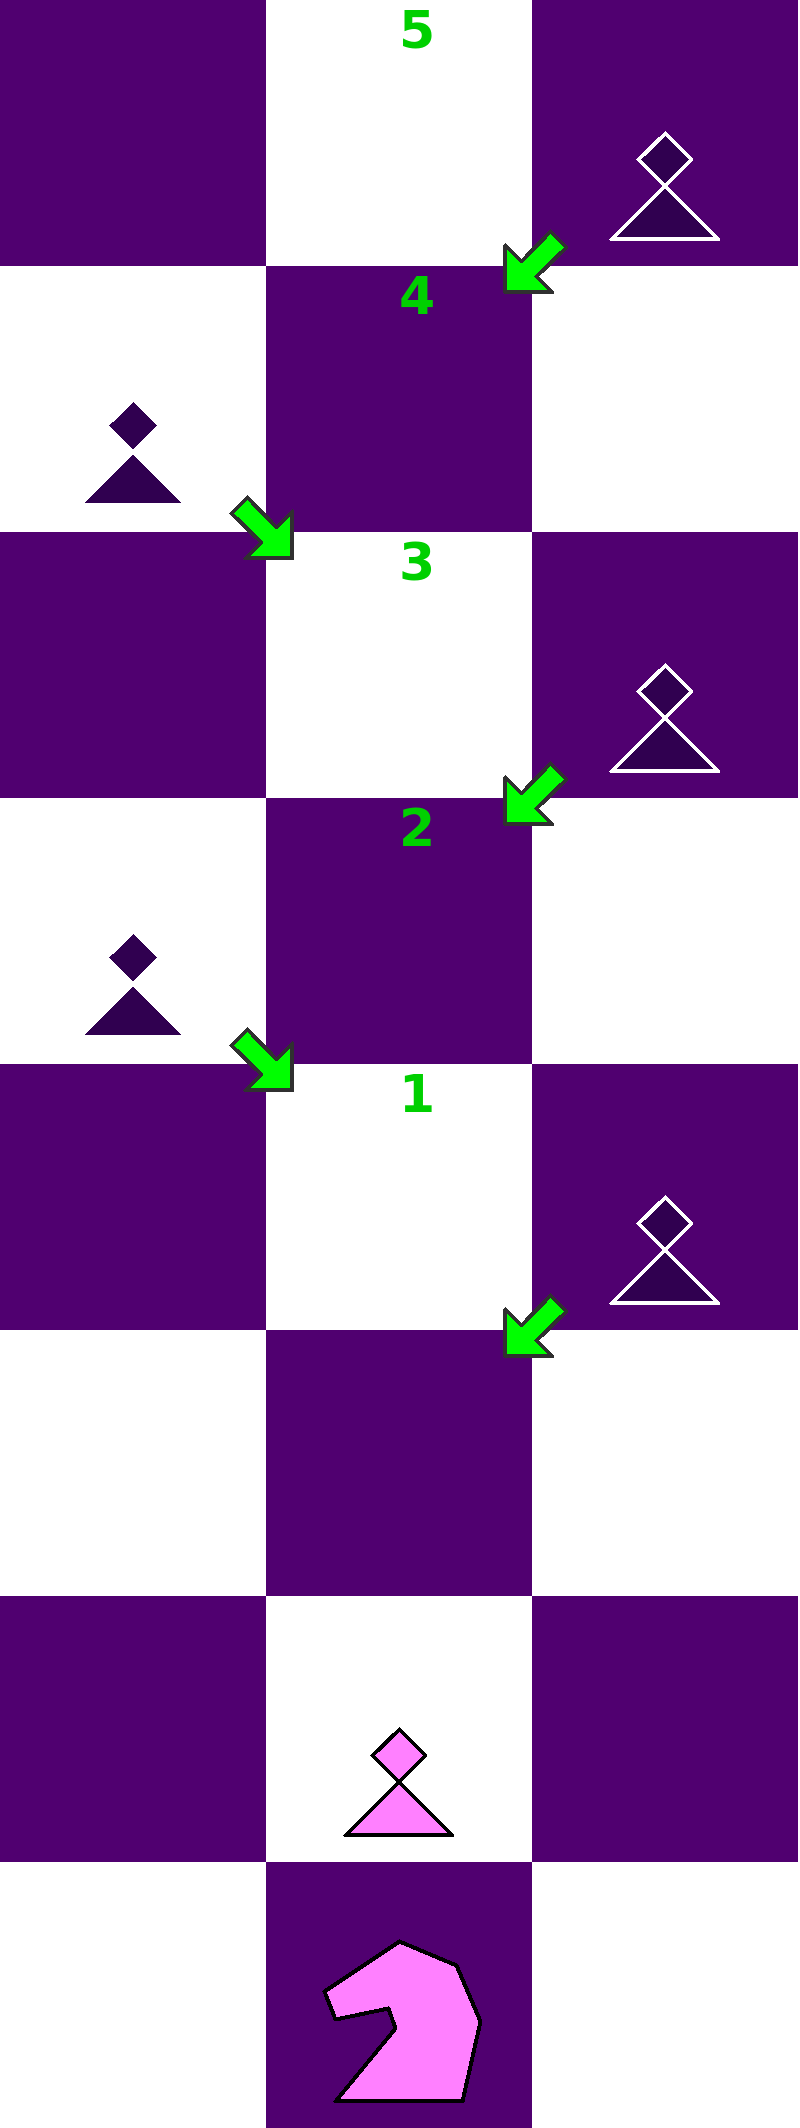
\includegraphics[width=0.1875\textwidth, keepaspectratio=true]{en_passants/10_miranda_s_veil_en_passant.png}
\caption{En passant}
\label{fig:10_miranda_s_veil_en_passant}
\end{wrapfigure}
Rush and en passant are identical to those in Classic Chess, only difference
is that Pawn can now move longer on initial turn, up to 6 fields in this
variant.

% \clearpage % ..........................................................

\vspace*{9.0\baselineskip}
\section*{Promotion}
\addcontentsline{toc}{section}{Promotion}

Promotion is non enforced, delayed variety, i.e. it's the same as in
\hyperref[sec:Age of Aquarius/Promotion]{previous chess variant}, Age of Aquarius.

\clearpage % ..........................................................

\section*{Castling}
\addcontentsline{toc}{section}{Castling}

Castling is the same as in Classical Chess, only difference is that King can move between 2 and 6 fields across.
All other constraints from Classical Chess still applies.

\noindent
\begin{figure}[!h]
\includegraphics[width=1.0\textwidth, keepaspectratio=true]{castlings/10_mv/miranda_s_veil_castling.png}
\caption{Castling}
\label{fig:miranda_s_veil_castling}
\end{figure}

In example above, all valid King's castling moves are numbered.

\noindent
\begin{figure}[!h]
\includegraphics[width=1.0\textwidth, keepaspectratio=true]{castlings/10_mv/miranda_s_veil_castling_right_05.png}
\caption{Castling long right}
\label{fig:miranda_s_veil_castling_right_05}
\end{figure}

In this example King was castling long to the right. Initial King's position is marked with "K".
After castling is finished, right Rook ends up at field immediately left to the King.

\clearpage % ..........................................................

\section*{Initial setup}
\addcontentsline{toc}{section}{Initial setup}

Compared to initial setup of Age of Aquarius, Wave is inserted between Knight and Unicorn
symmetrically, on both sides of chessboard. This can be seen in the image below:

\noindent
\begin{figure}[h]
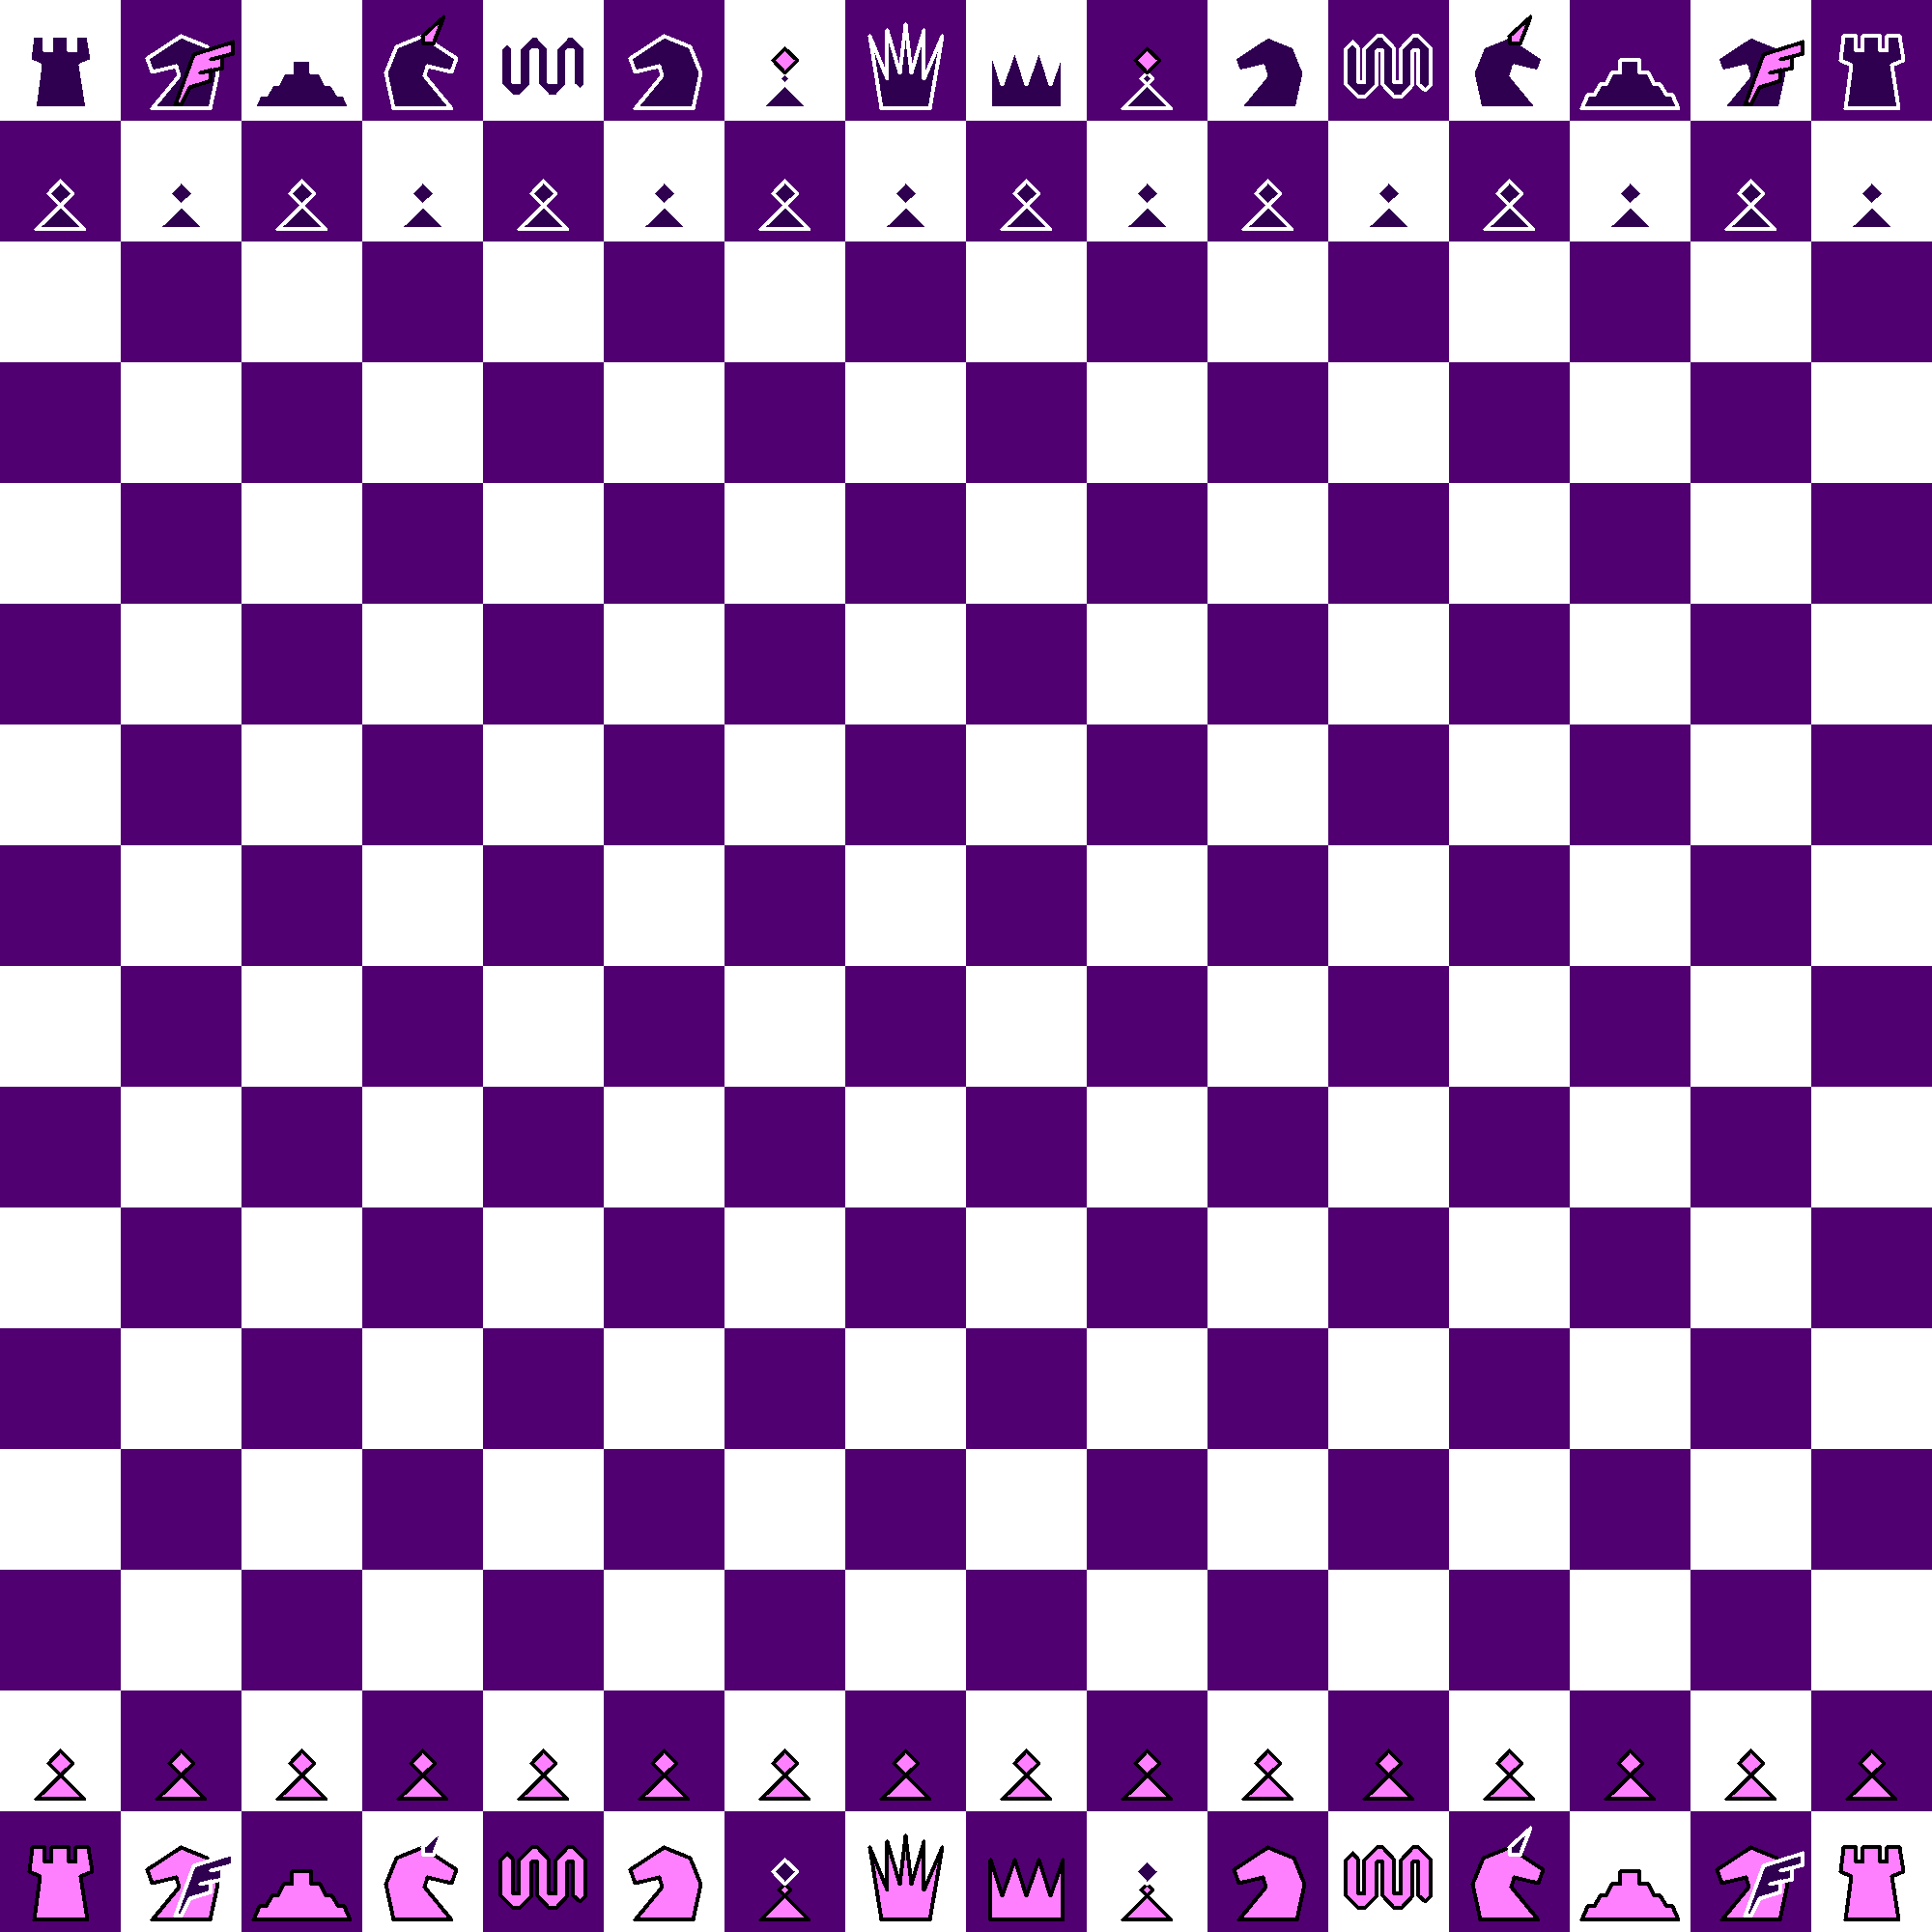
\includegraphics[width=1.0\textwidth, keepaspectratio=true]{boards/10_miranda_s_veil.png}
\caption{Miranda's veil board}
\label{fig:10_miranda_s_veil}
\end{figure}

\clearpage % ..........................................................
% ============================================== Miranda's veil chapter
